% we need a two-column format for the final report
\documentclass[12pt,twocolumn]{article}

\usepackage{graphicx}
\usepackage{amsmath}
\usepackage{float}

\usepackage{hyperref}

% chktex-file 44

\hypersetup{
    colorlinks=true,
    linkcolor=black,
    filecolor=magenta,      
    urlcolor=blue,
}

\title{ECS 171 Project Report\\\textit{Group 3}}
\author{Latif, Wahad (Leader)\\ Childs, Bradley\\Li, Siu Sing\\Natu, Neerja\\Niu, Kuangzhong}

\begin{document}
\maketitle
\tableofcontents
\newpage
\section{Introduction}
Modern life is dominated by companies knowing what you do. From your Instagram posts to your credit card statement, corporations love to collect your data. This data can not only used for business analysis or targeted advertising, but also for credit scores. This one number can determine whether you can get a loan, buy a house, or even get a job. Companies have a vested interest in making sure that this number is both accurate and hard to predict. If people learned how to game the system, it could lead to a loss of trust in the system. However, this also means that the system could be biased against certain groups of people.

In order to effectively minimize credit risk, it is important to conduct a reasonable evaluation of personal credit. A machine learning model that can give lenders a credit rating based on a vast collection of borrower's personal information and historical records is necessary. They may even extend beyond data that is traditionally used, analyzing social media posts to get a sense of a person's lifestyle beyond their financial history. This could lead to more accurate credit scores, but it could also lead to more bias and discrimination.

In the future, it may be the case that credit scores are calculated  by machine learning models. While potentially being more accurate, this could introduce many of the problems with bias and positive feedback loops that we see in other machine learning models. Therefore, it is important to understand how these models work and how they can be improved. It may also be important to provide tools to help people better understand what factors affect their credit score the most, and how they could improve their credit score.

Our goal is to take small steps towards this future by training models to predict credit scores based on a dataset of personal information and historical records. We will also analyze the results of these models to determine which factors are most important in determining credit score. Finally, we will discuss how these models could be improved and how they could be used in the future. Our hope is that our work will help people better understand how credit scores are calculated and how they can be improved.

\section{Literature Review}
In recent years, Machine Learning Models have gained popularity in the financial industry for their accuracy in predicting trends with large, complex data. To keep up with the increasing demand for more sophisticated fraud detection software, anti-money laundering systems, and risk detection programs, many big credit institutions have decided to deploy various ML models. 

In a study conducted by Vidovic et. al, ML algorithms were used to predict PD, the probability of default, which is a major component in risk assessment. Using annual financial data from private companies, attributes that are relevant in the calculation of PD, such as profitability, leverage, efficiency, Country Risk Score (CRS), and Industry Risk Score (IRS), were identified. They compared the performance of various models, such as Altman Z-score, Logistic Regression, SVM, Naive Bayes, and Decisions Trees, on data from private companies, and used ROC and AUC curves to determine performance statistics. Through this, they were able to determine that both logistic regression and decision tree models proved to have high accuracy at predicting PD values in the given dataset, with logistic regression achieving an accuracy rate of 93.1\% in-sample and 93.6\% for out-sample and decision trees achieving an accuracy rate of 99.8\% in-sample and 94.8\% out-sample. 

The results of this study were able to demonstrate the potential of ML models in predicting elements of credit risk scores. However, the researchers involved in this study also highlight the limitations of both their study, as well as ML models in predicting credit risk. They mention that the current dataset solely consists of values from private companies, and in the future, these models would have to be tested on larger and more diverse datasets. In addition, they acknowledge the fact that the larger datasets can contain a lot of noise, which could result in false predictions, and thus state that the correct precautions must be taken to account for this. 



\section{Data}
\subsection{Data Source}
We chose to use the German Credit Data Set from the UCI Machine Learning Repository. This dataset contains 1000 instances of credit applicants, each with 20 attributes. The attributes are a mix of numerical and categorical data. The dataset also contains a binary label indicating whether the applicant is a good or bad credit risk. The dataset was originally collected by Professor Dr. Hans Hofmann of the University of Hamburg. The dataset was donated to the UCI Machine Learning Repository in 1994. The dataset can be found at \href{https://archive.ics.uci.edu/ml/datasets/statlog+(german+credit+data)}{this link}.

\subsection{Data Preprocessing}
We had several key problems to overcome with our data processing. The first was that the data was primarily categorical, and used special encodings to represent the categories. We thus had to take steps to convert this categorical data using either numeric or one-hot encoding. 

\subsubsection{Numeric Encoding}
For many variables, such as employment history or amount of savings, it makes sense to provide an inherent numerical scale to the model. It pre-biases the models to expect these variables to be a range that has a definite positive and negative direction. It does not necessarily imply a correlation with the credit score, but it does provide a more intuitive way for the model to understand the data.

\subsubsection{One-Hot Encoding}
For other variables, however, we had no choice but to use one-hot encoding. For example, a person's sex and marital status. These variables have no inherent numerical scale, so we chose to use one-hot encoding to represent them. For one variable, the purpose of the loan, we did not choose to use this encoding scheme. This was because there were 10 possible values, and this would have added greatly to the dimensionality of the data. Instead, we found that splitting the dataset into 10 separate problems based on the purpose of the loan was a better solution. This was not entirely foolproof, as we did have issues with some datasets being prohibitively small, but we will discuss this more in later sections.

\section{Models}
We chose to make three models for this project:
\begin{itemize}
    \item Logistic Regression
    \item Random Forest
    \item Neural Network (Multilayer Perceptron)
\end{itemize}

\subsection{Logistic Regression}

We chose to use logistic regression as one of our models because it is a simple model that is easy to interpret. It is also a good baseline model to compare our other models to. 
\subsubsection{Hyperparameter Tuning}
We tuned our hyperparameters according to Table~\ref{tab:logistic_regression_hyperparameters}. 
% 'C': [0.001, 0.01, 0.1, 1, 10, 100],
% 'penalty': ['l1', 'l2'],
% 'solver': ['liblinear', 'saga'],
% 'fit_intercept': [True, False],
% 'tol': [1e-3, 1e-4, 1e-5],
\begin{table}
    \centering
    \begin{tabular}{|c|c|}
        \hline
        Parameter & Values \\
        \hline
        \hline
        C & 0.001, 0.01, 0.1, 1, 10, 100 \\
        \hline
        penalty & l1, l2 \\
        \hline
        solver & liblinear, saga \\
        \hline
        fit\_intercept & True, False \\
        \hline
        tol & 1e-3, 1e-4, 1e-5 \\
        \hline
    \end{tabular}
    \caption{Hyperparameters for Logistic Regression}\label{tab:logistic_regression_hyperparameters}
\end{table}

The best hyperparameters for each of the models we made are shown in Table~\ref{tab:logistic_regression_best_hyperparameters}. \texttt{fit\_intercept} was always true in the best results, so it was excluded from the table.


\begin{table}
    \centering
    \begin{tabular}{|c|c|}
        \hline
        Purpose & C, penalty, solver, tol \\
        \hline
        \hline
        Business & 0.01, l2, liblinear, 1e-3 \\
        \hline
        New Car & 1, l2, saga, 1e-4 \\
        \hline
        Used Car & 0.1, l2, saga, 1e-3 \\
        \hline
        Education & 0.001, l2, liblinear, 1e-3 \\
        \hline
        Furniture & 0.1, l2, liblinear, 1e-3 \\
        \hline
        Radio/TV & 1, l1, liblinear, 1e-3 \\
        \hline
        Repairs & 0.001, l1, liblinear, 1e-3 \\
        \hline
    \end{tabular}
    \caption{Best Hyperparameters for Logistic Regression}\label{tab:logistic_regression_best_hyperparameters}
\end{table}


\subsubsection{Results}
Because of the decision to split the dataset into  separate training tasks, we have separate models. The final results of these models are shown in Table~\ref{tab:logistic_regression_results}. These results are overall quite good, with the worst accuracy being 60\% and the worst MSE being 0.4. However, it is important to note that several of the datasets were quite small, and this caused issues for several other models that were even too small to be trained. This is a problem that we will discuss in later sections.

\begin{table}
    \centering
    \begin{tabular}{|c|r|r|}
        \hline
        Purpose & Accuracy & MSE \\
        \hline
        \hline
        Business & 0.750 & 0.250 \\
        \hline
        New Car & 0.702 & 0.298 \\
        \hline
        Used Car & 0.952 & 0.048 \\
        \hline
        Education & 0.600 & 0.400 \\
        \hline
        Furniture & 0.730 & 0.270 \\
        \hline
        Radio/TV & 0.839 & 0.161 \\
        \hline
        Repairs & 0.800 & 0.200 \\
        \hline
    \end{tabular}
    \caption{Results for Logistic Regression}\label{tab:logistic_regression_results}
\end{table}

\subsection{Random Forest}
\subsubsection{Hyperparameter Tuning}
% param_grid = {
%     'n_estimators': [50, 100, 150, 300],
%     'min_samples_split': [2, 5, 10],
%     'min_samples_leaf': [1, 2, 3],
%     'criterion': ['gini']
% }
We tuned our hyperparameters according to Table~\ref{tab:random_forest_hyperparameters}. The best hyperparameters for each of the models we made are shown in Table~\ref{tab:random_forest_best_hyperparameters}. \texttt{'gini'} was always the best criterion, so it was excluded from the table.
\begin{table}
    \centering
    \begin{tabular}{|c|c|}
        \hline
        Parameter & Values \\
        \hline
        \hline
        n\_estimators & 50, 100, 150, 300 \\
        \hline
        min\_samples\_split & 2, 5, 10 \\
        \hline
        min\_samples\_leaf & 1, 2, 3 \\
        \hline
        criterion & gini \\
        \hline
    \end{tabular}
    \caption{Hyperparameters for Random Forest}\label{tab:random_forest_hyperparameters}
\end{table}

\begin{table}
    \centering
    \begin{tabular}{|c|c|}
        \hline
        Purpose & estimators, split, leaf \\
        \hline
        \hline
        Appliance & 50, 5, 1 \\
        \hline
        Business & 300, 5, 2 \\
        \hline
        New Car & 50, 2, 3 \\
        \hline
        Used Car & 100, 2, 1 \\
        \hline
        Education & 50, 2, 3 \\
        \hline
        Furniture & 300, 2, 2 \\
        \hline
        Other & 50, 2, 1 \\
        \hline
        Radio/TV & 150, 5, 1 \\
        \hline
        Repairs & 50, 2, 2 \\
        \hline
    \end{tabular}
    \caption{Best Hyperparameters for Random Forest}\label{tab:random_forest_best_hyperparameters}
\end{table}
\subsubsection{Results}

We recorded the accuracy and MSE for each of the models we made. These results are shown in Table~\ref{tab:random_forest_results}.


\begin{table}
    \centering
    \begin{tabular}{|c|r|r|}
        \hline
        Purpose & Accuracy & MSE \\
        \hline
        \hline
        Appliance & 0.667 & 0.333 \\
        \hline
        Business & 0.750 & 0.250 \\
        \hline
        New Car & 0.809 & 0.191 \\
        \hline
        Used Car & 0.904 & 0.095 \\
        \hline
        Education & 0.500 & 0.500 \\
        \hline
        Furniture & 0.702 & 0.297 \\
        \hline
        Other & 0.333 & 0.667 \\
        \hline
        Radio/TV & 0.768 & 0.232 \\
        \hline
        Repairs & 0.400 & 0.600 \\
        \hline
    \end{tabular}
    \caption{Results for Random Forest}\label{tab:random_forest_results}
\end{table}


\subsection{Neural Network (Multilayer Perceptron)}
Neural networks, in particular simple perceptron models seemed ideal for the type of data we selected. We had a relatively small set of inputs, and a single binary output. We did not end up splitting the model into separate categories because the dataset of 1000 entries all together was barely large enough to train a neural network.

\subsubsection{Results}
\figure[htbp]
    \centering
    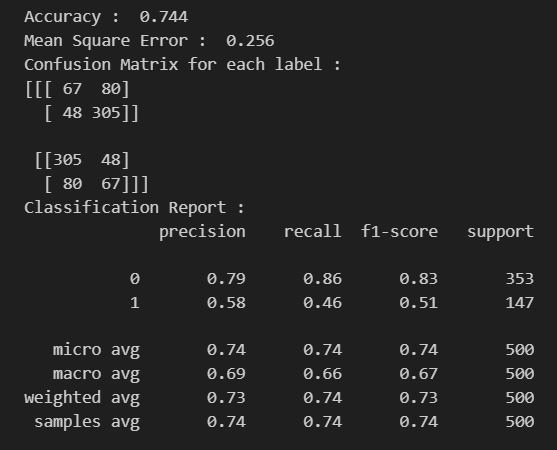
\includegraphics[width=0.5\textwidth]{images/nn_results.png}
    \caption{Results for Neural Network}\label{fig:nn_results}
\endfigure
We achieved an accuracy of 0.744 and an MSE of 0.256. This is not as good as the other models, but it is still a reasonable result. Because this model is not split by purpose, the dimensionality is much higher, which may have contributed to the lower accuracy. Since the model is much more likely to overfit, we chose early stopping to prevent this. 

\section{Conclusion and Overview}
\subsection{Comparing Models}
Since we had a split in how we were able to train and process our models, it can become difficult to directly compare results between our three models. We chose to look at the \texttt{new car} dataset in order to compare them, since it was large and had good results for all three models. \ref{fig:logistic_newcar_results} shows the results for the logistic regression model and \ref{fig:randomforest_newcar_results} shows the random forest model.
\begin{figure}
    \centering
    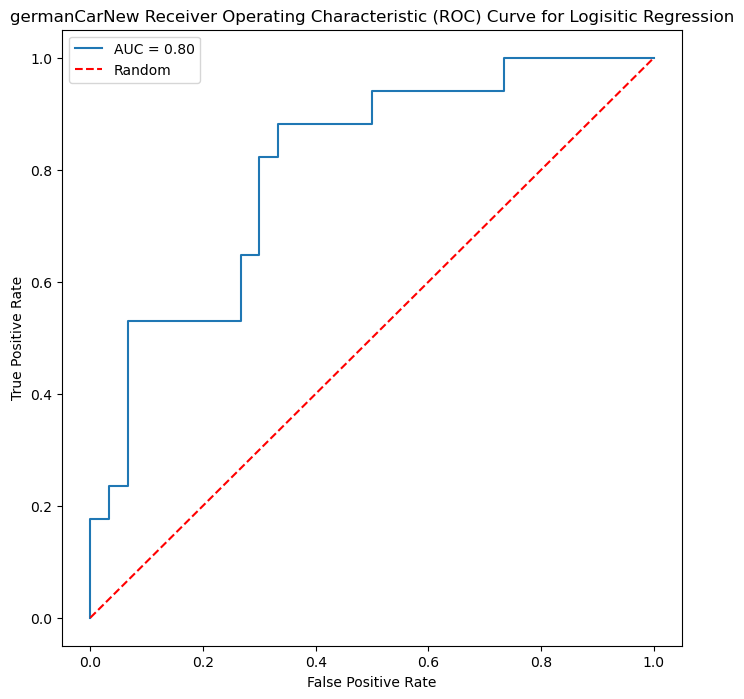
\includegraphics[width=0.5\textwidth]{images/logistic_newcar.png}
    \caption{Logistic Model Results for New Car Dataset}\label{fig:logistic_newcar_results}
\end{figure}

\begin{figure}
    \centering
    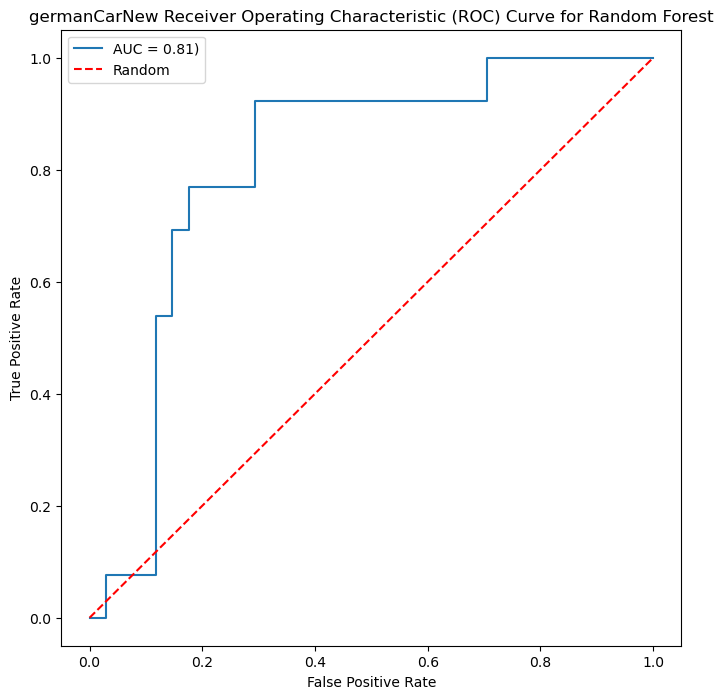
\includegraphics[width=0.5\textwidth]{images/randomforest_newcar.png}
    \caption{Random Forest Model Results for Random Forest}\label{fig:randomforest_newcar_results}
\end{figure}

Random Forest proved to be the most effective in this comparison, with our neural network model coming in second and logistic in last. This is not entirely surprising, as logistic regression is a relatively simple model. Our largest issue was the size of our dataset, which was not large enough to train a neural network effectively. If the dataset was larger, we would expect the neural network to perform better than the random forest model.


\subsection{Overall Sucess}
We think that we achieved the goals that we established when we began this project. We discovered some of the issues that may arise when trying to implement credit score calculations on a large, commercial scale, and we were able to train models that could predict credit scores with reasonable accuracy.

\subsection{Looking Forward and Improvements}
Our main takeaway for future research is that a better dataset is needed. The dataset we used was too small to train a neural network effectively, and it was too small to split into separate datasets for each purpose. It is reasonable to expect that any companies trying to use this will have access to datasets many orders of magnitude larger. But we also saw that even small datasets can produce predictions that are accurate enough to be useful. It may also be interesting to explore more types of models in the future, such as support vector machines.


\end{document}